\chapter{Conceitos e revisão bibliográfica}
\label{chap:estadodaarte}

Uma visão geral sobre agrupamentos é apresentada na seção \ref{agrupamentos}. Na seção \ref{dbscan} apresenta-se o algoritmo DBSCAN em detalhes e suas características. A seção \ref{stdbscan} apresenta o ST-DBSCAN, que é utilizada nesse trabalho para auxiliar os métodos de previsão dinâmica. Na seção  \ref{chap:redes-dinamicas}  discute-se redes dinâmicas e exibe-se o modelo Dynagraph e um editor de características. A seção  \ref{chap:trabalhos-relacionados}  define e apresenta os trabalhos relacionados ao problema de agrupamentos dinâmicos.

\section{Agrupamentos}
\label{agrupamentos}

A técnica de agrupamento, também chamada de \textit{clustering}, é uma das técnicas de mineração de dados mais comuns e é usada para descobrir padrões de distribuição nos dados. O agrupamento é feito com base na similaridade das características e na posição dos objetos. Dessa maneira, o objetivo é que os objetos do mesmo grupo sejam muito similares entre si e muito diferentes dos objetos de outros grupos.

Essa técnica é muito utilizada para dados estáticos. No entanto, há poucos trabalhos no âmbito espaço-temporal onde os dados estão na forma de campos espaço-temporais contínuos e os agrupamentos são dinâmicos. Além disso, os dados espaço-temporais originados por satélites em órbita terrestre, telefones celulares e outros sensores tendem conter muitos ruídos, são incompletos e heterogêneos, tornando sua análise especialmente desafiadora \cite{faghmous2013}.

Agrupamentos dinâmicos podem mudar seu tamanho, forma, localização e propriedades estatísticas de um tempo para o próximo. Embora os agrupamentos possam se mover ou mudar de forma, existem vários pontos que não alteram as associações de grupos por um período de tempo. Tendo isso em vista é possível extrair de forma autônoma agrupamentos dinâmicos em dados espaço-temporais contínuos que podem conter valores, ruídos ou características muito variáveis.

Existem muitas variações quanto à formação de grupos. Pode-se querer definir grupos a partir de um processo onde é dado o número desejado de partições a serem aplicadas entre os objetos a serem agrupados; pode-se querer definir quais são os grupos que naturalmente se formam dentro de um conjunto dado de objetos; pode-se querer classificar objetos a partir de classes de objetos já conhecidas; e por fim pode-se querer identificar objetos que não correspondem a nenhum grupo. 

Em processos de agrupamento dinâmico é necessário conhecer como os objetos se agrupam naturalmente assim como identificar os objetos que não estão associados a qualquer desses grupo.

Os métodos mais tradicionais para esses casos estão na classe dos métodos denominados particionais e hierárquicos. Alguns algoritmos de agrupamento integram as idéias de vários outros, logo é difícil classificar um algoritmo pertencendo a somente uma categoria de métodos de agrupamento. Além do que, algumas aplicações podem ter critérios que necessitam a integração de várias técnicas de agrupamento. Os principais métodos de agrupamento existentes na literatura são categorizados, como mostram as próximas sessões.

\subsection{Métodos baseados em particionamento}
A ideia principal desta classe de algoritmos de agrupamentos é criar ${K}$ grupos dos dados, onde ${K}$ é inserido pelo usuário.
Esse método consiste em escolher ${K}$ objetos como sendo os centros dos ${K}$ grupos.
Os objetos são divididos entre os ${K}$ grupos de acordo com algum critério de similaridade
estabelecido pelo algoritmo, de modo que cada objeto fique no grupo que tem o menor valor de
distância entre o objeto e o centro do grupo a que ele pertence.
Os algoritmos de particionamento são muito populares devido à sua facilidade de implementação e baixo custo computacional; no entanto, eles têm essas desvantagens: (1) eles são sensíveis à presença de ruído e \textit{outliers}, (2) eles podem descobrir apenas grupos com formas convexas e (3) o número de grupos precisa ser especificado.


\subsubsection{Agrupamentos K-Médias}
O algoritmo de agrupamento k-médias é uma das técnicas mais conhecidas dessa abordagem e foi introduzido por \cite{Macqueen67}. Ele utiliza a média dos objetos que são do grupo em questão, também conhecido como centro geométrico do grupo. A idéia principal neste algoritmo é usar a média dos objetos para atribuí-los a grupos e também usá-los para  representá-los.
K-médias é um algoritmo que garante a convergência para um ótimo local, mas não necessariamente um ótimo global. À medida que ${K}$ aumenta, o custo de encontrar a solução ótima diminui, e atinge seu mínimo quando ${K}$ é igual ao número de objetos \cite{Wu2008}. Especificamente, o procedimento é mostrado abaixo:
 \begin{enumerate}
	\item Inserir os objetos para serem agrupados e também o número ${K}$ de grupos.
	\item Escolher aleatoriamente os ${K}$ objetos como centro dos grupos originais.
	\item Atribuir cada objeto ao grupo com a média mais próxima.
	\item Calcular a nova média de cada grupo.
	\item Repetir a partir do passo 3.
	\item Parar quando o critério de convergência estiver satisfeito. O critério mais frequentemente usado, é a minimização do erro quadrático, dado por: 
	\begin{equation}
	E = \sum_{i=1}^{k}\sum_{o\in C_{i}} |o - \mu_{i}|^{2}
	\end{equation}
	onde ${o}$ é o ponto no espaço representando um dado objeto, ${\mu_{i}}$ é o representante do grupo ${C_{i}}$,
	 e ${K}$ o número de grupos.
\end{enumerate}

A seguir um exemplo do funcionamento do algoritmo na figura \ref{fig:kmedias}. Os objetos são mostrados como pontos e os centróides dos grupos são mostrados como cruzes. Na etapa \ref{fig:kmedias}-(a) encontra-se o conjunto de dados original. Em \ref{fig:kmedias}-(b) os centróides dos grupos são escolhidos aleatoriamente. De \ref{fig:kmedias}-(c) até \ref{fig:kmedias}-(f) ilustra a execução de duas iterações do k-médias. Em cada iteração, atribui-se cada objeto ao centróide mais próximo. Em seguida, cada centróide é movido para a média dos pontos atribuídos a ele.
\begin{figure}[!ht]
	\centering
	\Caption{\label{fig:kmedias} K-médias}	
	\UECEfig{}{
		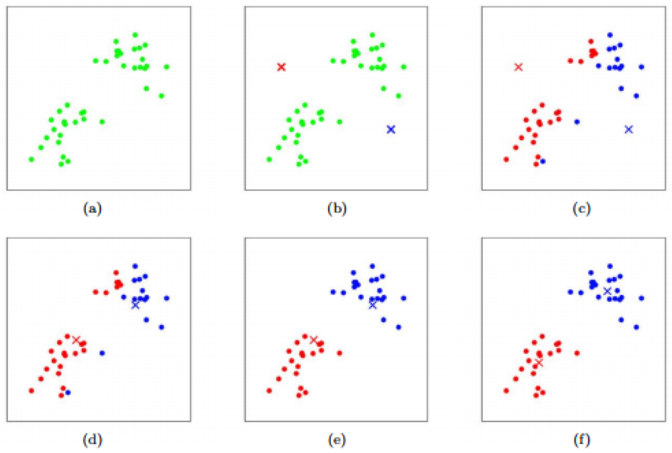
\includegraphics[width=14cm]{figuras/k-medias.png}
	}{
		\Fonte{\cite{kmedias:exemplo}}
	}
\end{figure}

\subsubsection{Agrupamentos K-Medoids}
O algoritmo de \textit{K-Medoids} ou K-medianas foi introduzido primeiramente em \cite{kaufmann1990}. Seu objetivo é particionar os objetos em ${k}$ grupos, previamente conhecidos, tal que a soma das distâncias entre cada objeto e a mediana do seu grupo seja mínima. Nesse algoritmo, cada grupo é representado pelo objeto mais próximo ao centro, conhecido também por \textit{medoid}.
O processo geral para o algoritmo é o seguinte:
 \begin{enumerate}
 	\item Escolher aleatoriamente ${k}$ objetos como os \textit{medoids} iniciais.
 	\item Atribuir cada um dos objetos restantes ao grupo que com o \textit{medoid} mais próximo.
 	\item Em um grupo, selecionar aleatoriamente um objeto que não seja \textit{medoid} (${nonmedoid}$), que será referenciado como ${O_{nonmedoid}}$.
 	\item Calcular o custo de substituir o \textit{medoid} com ${O_{nonmedoid}}$. Este custo é a diferença do erro quadrático se o \textit{medoid} atual for substituído por ${O_{nonmedoid}}$. Se for negativo, fazer ${O_{nonmedoid}}$ o \textit{medoid} do grupo. O erro quadrático é novamente somado ao erro de todos os objetos:
 	\begin{equation}
 	E = \sum_{i=1}^{k}\sum_{o\in C_{i}} |o - O_{medoid(i)}|^{2}
 	\end{equation}
 	onde ${O_{medoid(i)}}$ é o \textit{medoid} do grupo ${C_{i}}$.
 	\item Repetir a partir do passo 2 até que não haja mudanças. 
 \end{enumerate}

Um exemplo é dado nas figuras \ref{fig:kmedianaA} e \ref{fig:kmedianaB}, onde nove objetos são distribuídos em dois grupos, portanto dois \textit{medoids}. Os objetos azuis correspondem aos \textit{medoids}, os segmentos de reta são as distâncias implícitas ao medoid de cada grupo, e os valores S1 e S2 são às somas das distâncias dos objetos aos seus respectivos \textit{medoids}. Nota-se que a figura \ref{fig:kmedianaB} representa a melhor solução, pois a soma total é igual a 300.

\begin{figure}[!ht]
	\centering
	\Caption{\label{fig:kmedianaA} K-mediana (a)}	
	\UECEfig{}{
		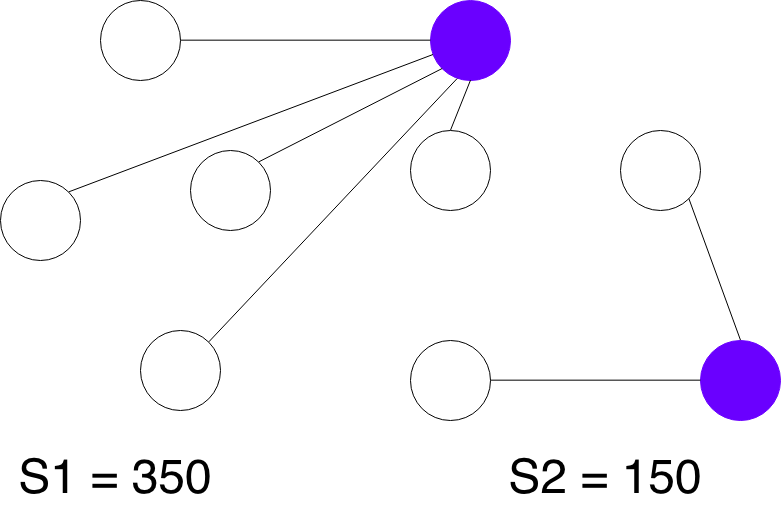
\includegraphics[width=7cm]{figuras/k-mediana-a.png}
	}{
		\Fonte{Elaborado pelo autor}
	}
\end{figure}
\begin{figure}[!ht]
	\centering
	\Caption{\label{fig:kmedianaB} K-mediana (b)}	
	\UECEfig{}{
		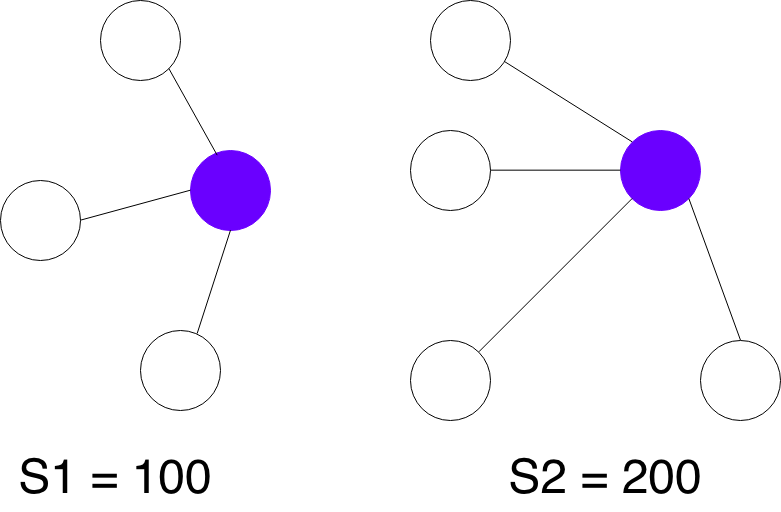
\includegraphics[width=7cm]{figuras/k-mediana-b.png}
	}{
		\Fonte{Elaborado pelo autor}
	}
\end{figure}

\subsection{Métodos Hierárquicos}
Nesta classe de algoritmos os objetos são colocados em uma hierarquia que é percorrida de baixo para cima (\textit{bottom-up}) ou de cima para baixo (\textit{top-down}) para criar os grupos. A vantagem deste tipo de agrupamento é que ele não requer nenhum conhecimento sobre o número de grupos, e a desvantagem é sua complexidade computacional \cite{Lin2004}. Muitas vezes, uma estrutura em árvore, um dendrograma, é usada para representar os níveis hierárquicos aninhados.

Os métodos aglomerativos funcionam de uma maneira \textit{bottom-up},
assumindo inicialmente que cada elemento do conjunto de dados representa um grupo. Em seguida, os grupos são fundidos em grupos maiores até a criação de um grupo único ou qualquer outro critério de parada.

A abordagem divisiva trabalha de maneira \textit{top-down}, considerando todo o conjunto de dados como um só grupo, que é dividido de maneira recursiva de acordo com a medida (métrica) de similaridade estabelecida.

\subsubsection{O algoritmo BIRCH}
\label{sub:birch}

Em \cite{Zhang1996}, BIRCH significa balanceamento interativo com redução e agrupamento usando hierarquias - \emph{Balanced Iterative Reducing and Clustering using Hierarchies}. Ele é um algoritmo usado para agrupamentos em bases de dados muito grandes sendo considerado um dos métodos hierárquicos mais utilizados pela literatura. As vantagens do BIRCH são as seguintes:

\begin{itemize}
	\item BIRCH trabalha de maneira local. Isso é obtido usando medições que indicam a proximidade natural dos pontos, de modo que cada decisão de agrupamento possa ser feita sem verificar todos os pontos de dados ou grupos existentes.
	\item Leva em conta a estrutura de dados espacial. Ele trata os pontos em uma região densa como um único grupo, enquanto os pontos em uma região esparsa são caracterizados como \textit{outliers} e podem ser removidos opcionalmente.
	\item O algoritmo faz uso da memória disponível enquanto minimiza os custos de Entrada/Saída de dados.
\end{itemize}

Os principais conceitos do BIRCH, que funcionam de maneira incremental são: o Agrupamento por Característica (AC) e AC-árvore. Onde AC consiste em tomar todas as informações que precisam ser mantidas sobre um grupo. Já o AC-árvore é utilizado para representar a hierarquia de grupos.

A estrutura da AC-árvore é exibida na figura \ref{fig:birch} e descrita a seguir.

\begin{itemize}
    \item Cada nó que não é folha tem no máximo ${B}$ entradas;
    \item Cada nó folha tem no máximo ${L}$ AC entradas que satisfazem o limite ${T}$, que é o diâmetro máximo de raio;
    \item P (tamanho da página em bytes) é o tamanho máximo de um nó;
    \item Compacto: cada nó da folha é um subgrupo, não um ponto de dados;
\end{itemize}

\begin{figure}[!ht]
	\centering
	\Caption{\label{fig:birch} Estrutura de uma AC-árvore}	
	\UECEfig{}{
		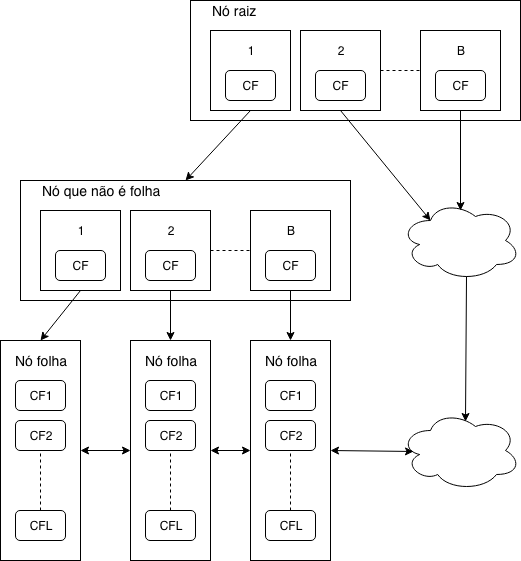
\includegraphics[width=14cm]{figuras/Birch.png}
	}{
		\Fonte{Elaborado pelo autor}
	}
\end{figure}

O agrupamento acontece essencialmente em duas fases. Na primeira delas, o algoritmo lê o conjunto de dados e constrói uma AC-árvore inicial. Essa árvore é utilizada para representar a hierarquia dos grupos. Na segunda fase, um algoritmo de agrupamento selecionado é aplicado às folhas da AC-árvore, removendo grupos esparsos e agrupando os mais densos em grupos maiores.

O algoritmo BIRCH é descrito como segue:

\begin{enumerate}
    \item Carregar os dados na memória através da construção de uma AC-árvore;
        \begin{enumerate}
            \item Escolher um valor inicial de entrada, começar inserindo os pontos de dados um por um na árvore conforme o algoritmo de inserção;
            \item Se, no meio da etapa acima, o tamanho da AC-árvore exceder o tamanho da memória disponível, aumentar o valor do limite;
            \item Converter a árvore parcialmente construída em uma nova árvore;
            \item Repetir as etapas acima até que todo o conjunto de dados seja verificado e uma árvore completa seja criada;
            \item Manipulação dos \textit{outliers};
        \end{enumerate}
    \item Condensar a AC-árvore anterior em uma menor;
        \begin{enumerate}
            \item Criar uma AC-árvore menor aumentando o limite;
            \item Remover mais \textit{outliers};
        \end{enumerate}
    \item Agrupamento global;
        \begin{enumerate}
            \item Aplicar o algoritmo nos dados de entrada da AC-árvore;
            \item Melhorar a qualidade dos grupos;
        \end{enumerate}    
    \item Aprimoramentos do agrupamento;
        \begin{enumerate}
            \item Verificar todo o conjunto de dados para rotular os pontos de dados;
            \item Manipulação dos \textit{outliers};
        \end{enumerate}    
\end{enumerate}

Um exemplo do Birch é dado a seguir na figura \ref{fig:birch01}. Após a inserção do subgrupo AC8 em LN1, e se o fator de ramificação de um nó folha não puder exceder 3, então o LN1 é dividido, como exibe a figura \ref{fig:birch02}. Se o fator de ramificação de um nó que não é folha não puder exceder 3, a raiz é dividida e a altura da AC-árvore aumenta em um, como mostra a figura \ref{fig:birch03}.

\begin{figure}[!ht]
	\centering
	\Caption{\label{fig:birch01} Exemplo algoritmo de Birch - Novo subgrupo}	
	\UECEfig{}{
		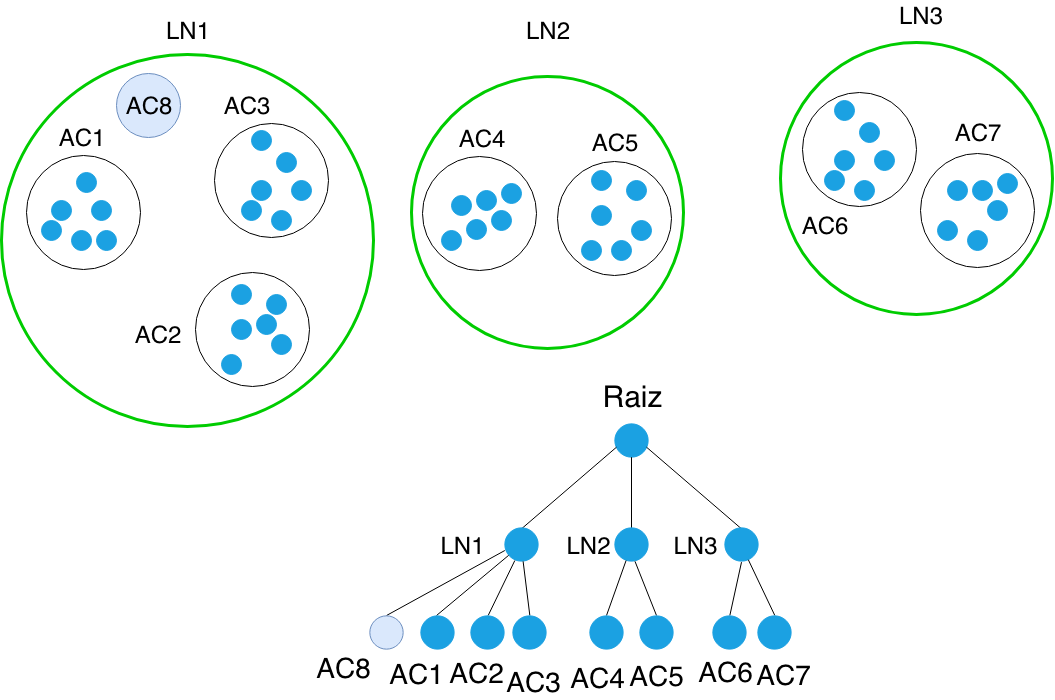
\includegraphics[width=14cm]{figuras/Birch01.png}
	}{
		\Fonte{Elaborado pelo autor}
	}
\end{figure}

\begin{figure}[!ht]
	\centering
	\Caption{\label{fig:birch02} Exemplo algoritmo de Birch - Operação de inserção parte 1}	
	\UECEfig{}{
		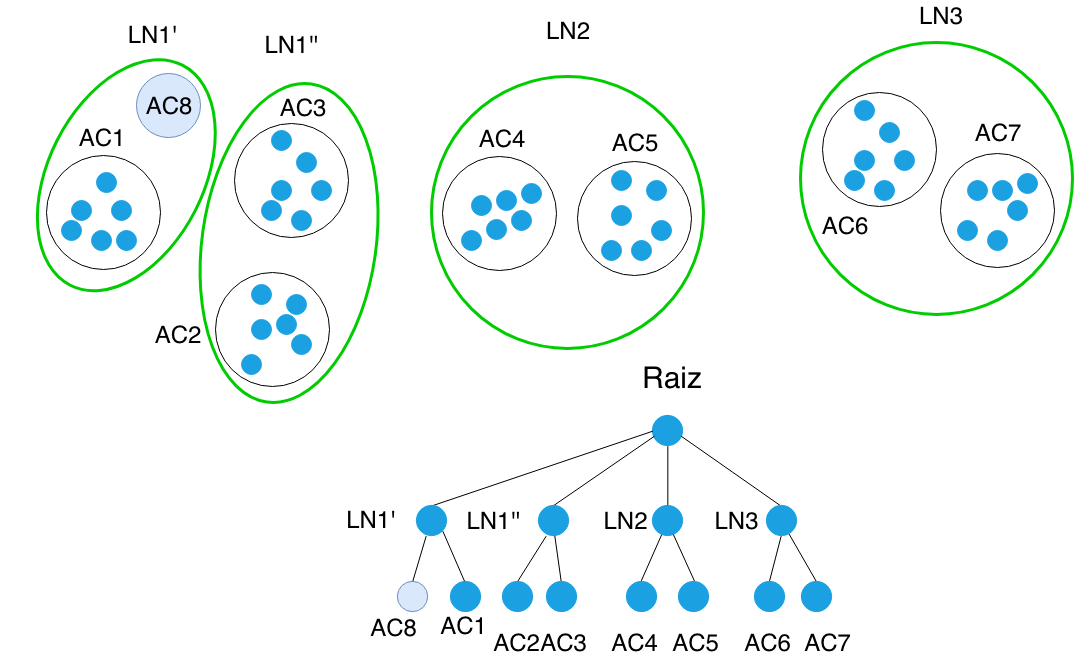
\includegraphics[width=14cm]{figuras/Birch02.png}
	}{
		\Fonte{Elaborado pelo autor}
	}
\end{figure}

\begin{figure}[!ht]
	\centering
	\Caption{\label{fig:birch03} Exemplo algoritmo de Birch - Divisão da raiz}	
	\UECEfig{}{
		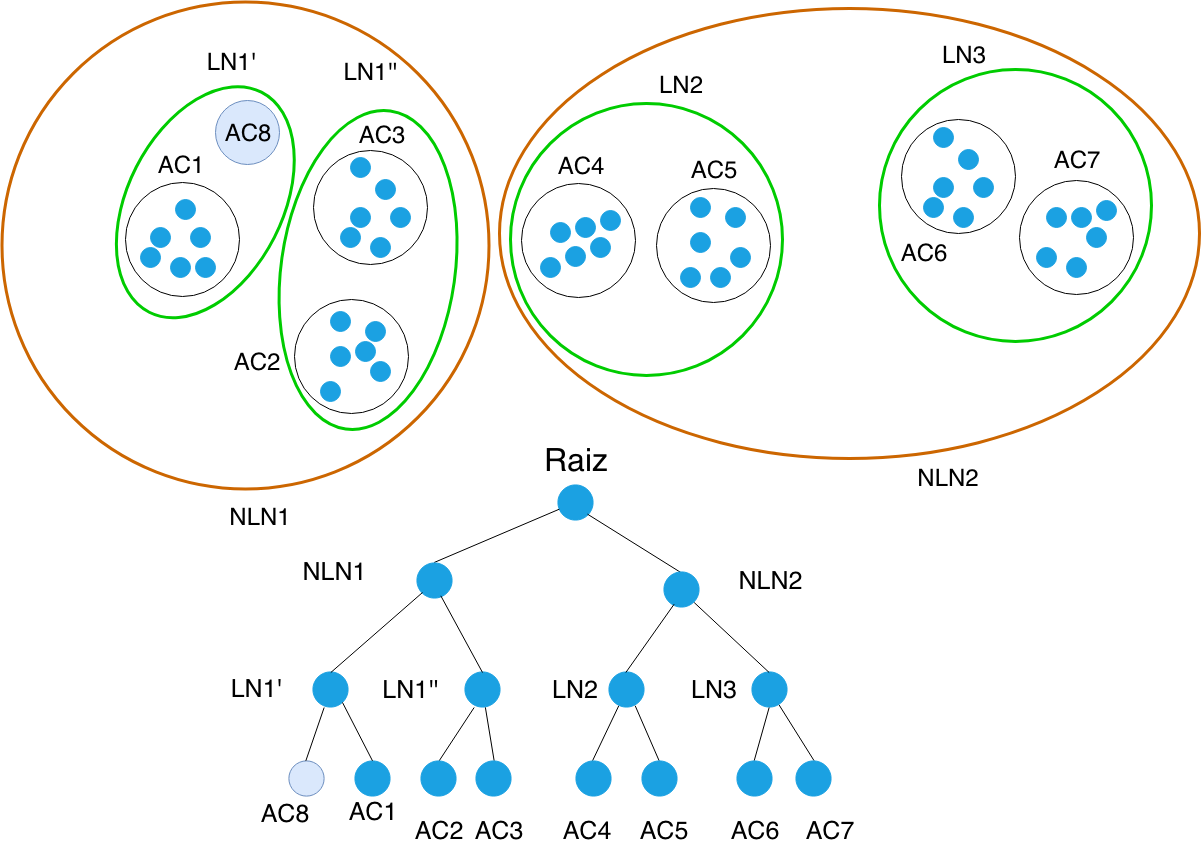
\includegraphics[width=14cm]{figuras/Birch03.png}
	}{
		\Fonte{Elaborado pelo autor}
	}
\end{figure}

\subsubsection{O algoritmo CURE}
Em \cite{Guha1998}, outro algoritmo hierárquico é proposto para detectar grupos que não são necessariamente convexos. Os grupos do CURE são representados por um número fixo de objetos bem espalhados que são encolhidos em direção ao centro do grupo por uma determinada fração. O CURE difere do algoritmo BIRCH de duas maneiras:
\begin{itemize}
\item O CURE começa desenhando uma amostra aleatória em vez de pré-agrupar todos os objetos de dados, como no caso do BIRCH.
\item O CURE primeiro particiona a amostra aleatória e, em seguida, em cada partição, os dados são parcialmente agrupados. Em seguida, os \textit{outliers} são eliminados e os dados pré-agrupados em cada partição são agrupados para gerar os grupos finais.
\end{itemize}
Os resultados experimentais no artigo mostram que o tempo de execução do CURE é sempre menor que o do BIRCH. Mais importante, os resultados mostram que, à medida que o tamanho do banco de dados aumenta, o tempo de execução do BIRCH aumenta rapidamente enquanto o tempo de execução do CURE aumenta muito pouco. O motivo disto é que o BIRCH varre todo o banco de dados e usa todos os objetos para o pré-agrupamento, enquanto o CURE usa apenas uma amostra aleatória.

As etapas do algoritmo CURE são:

\begin{enumerate}
    \item Seleção aleatória;
        \begin{enumerate}
            \item quando todo o conjunto de dados é considerado como entrada de algoritmo, o tempo de execução pode ser alto devido aos custos de I/O;
            \item para acelerar as operações do algoritmo, a amostragem aleatória é ajustada na memória principal;
        \end{enumerate}
    \item Particionamento;
        \begin{enumerate}
            \item Quando os grupos no conjunto de dados se tornam menos densos, a seleção aleatória com objetos limitados torna-se inútil, logo é necessário aumentar a amostragem aleatória;
            \item Cada grupo de objetos deve caber na memória principal para aumentar o desempenho do grupo parcialmente;
        \end{enumerate}
    \item Agrupamento parcial das partições;
        \begin{enumerate}
            \item Um número constante ${c}$ de objetos bem dispersos em um grupo é escolhido como representativo. Esses objetos capturam toda a forma possível que poderia ter o grupo;
            \item Os objetos são reduzidos em direção à média do grupo;
            \item Os grupos com o par de objetos representativos mais próximo são os grupos que são mesclados (merge) em cada etapa do CURE;
        \end{enumerate}
    \item Remoção dos ${outliers}$;
        \begin{enumerate}
            \item Os \textit{outliers}, devido à sua maior distância para outros objetos, tendem a se agrupar com outros objetos e geralmente crescem a uma taxa muito mais lenta do que os grupos atuais. Assim, o número de objetos em uma coleção de \textit{outliers} é normalmente muito menor que o número em um grupo.
        \end{enumerate}
    \item Agrupamento parcial dos grupos;
    \item Rotular dados no disco;
        \begin{enumerate}
            \item O processo de seleção aleatória do conjunto de dados inicial, exclui a maioria dos objetos.
            \item Estes objetos devem ser atribuídos a algum grupo criado em fases anteriores.
            \item Cada grupo criado é representado por uma fração de objetos selecionados aleatoriamente e cada objeto excluído na primeira fase é associado ao grupo cujo objeto representativo está mais próximo;
        \end{enumerate}
\end{enumerate}

As figuras \ref{fig:cureA}, \ref{fig:cureB}, \ref{fig:cureC} e \ref{fig:cureD} descrevem um exemplo do CURE.
\begin{figure}[!ht]
	\centering
	\Caption{\label{fig:cureA} CURE - amostra de dados}	
	\UECEfig{}{
		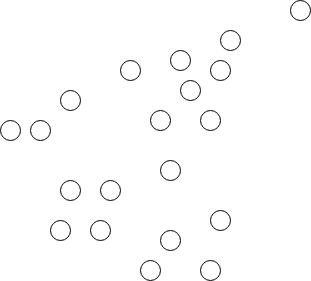
\includegraphics[width=6cm]{figuras/cureA.png}
	}{
		\Fonte{Elaborado pelo autor}
	}
\end{figure}
\begin{figure}[!ht]
	\centering
	\Caption{\label{fig:cureB} CURE - Três grupos com pontos representativos}
	\UECEfig{}{
		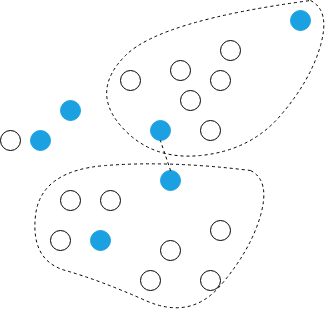
\includegraphics[width=6cm]{figuras/cureB.png}
	}{
		\Fonte{Elaborado pelo autor}
	}
\end{figure}
\begin{figure}[!ht]
	\centering
	\Caption{\label{fig:cureC} CURE - Merge dos grupos com pontos mais próximos}	
	\UECEfig{}{
		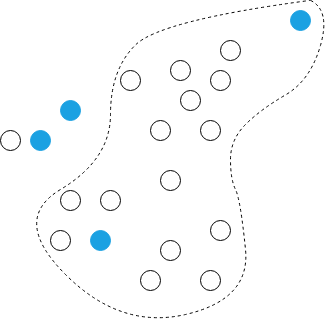
\includegraphics[width=6cm]{figuras/cureC.png}
	}{
		\Fonte{Elaborado pelo autor}
	}
\end{figure}
\begin{figure}[!ht]
	\centering
	\Caption{\label{fig:cureD} CURE - Encolhimento de pontos representativos}	
	\UECEfig{}{
		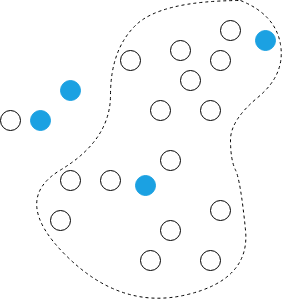
\includegraphics[width=6cm]{figuras/cureD.png}
	}{
		\Fonte{Elaborado pelo autor}
	}
\end{figure}

\subsubsection{Algoritmo de Kruskal}
Este algoritmo foi proposto em \cite{kruskal} e seu objetivo é encontrar um subconjunto das arestas que forma uma árvore geradora mínima que contém todos os vértices, onde a soma dos pesos das arestas da árvore é minimizada.

Seja ${G = (V, E)}$ um grafo convexo de ${V}$ vértices com o conjunto ${E}$ de arestas, o algoritmo de Kruskal inicia com T vazio e seleciona a aresta de ${E}$ que tem o menor peso e se ela conecta dois grupos distintos, então colocam-nas no conjunto ${T}$. Em seguida, os dois grupos formados se unem para formar um novo agrupamento, e se ela não conectar dois grupos diferentes, então a aresta é descartada. Com isso evita-se a formação de um ciclo. O algoritmo prossegue assim até obter um único grupo, neste caso ${T}$ constitui a solução.
Esse método é utilizado no algoritmo IGN apresentado na seção \ref{sub:ign} e seu funcionamento pode ser resumido nos seguintes passos:
\begin{enumerate}
    \item T = ${\varnothing}$;
    \item Para cada vértice ${v \in V[G]}$ criar as árvores;
    \item Colocar os arcos em ordem crescente de peso;
    \item Para cada arco $({u, v} \in E)$ verificar se ambos estão na mesma árvore. Senão, adicinar o arco em T e juntar os vértices nas duas árvores.
\end{enumerate}

A figura \ref{fig:kruskal} exibe os passos iterativos do algoritmo de Kruskal, que foi implementado no sistema SCLUSTER \cite{scluster}.

\begin{figure}[!ht]
	\centering
	\Caption{\label{fig:kruskal} Etapas iterativas do algoritmo de Kruskal}
	\UECEfig{}{
		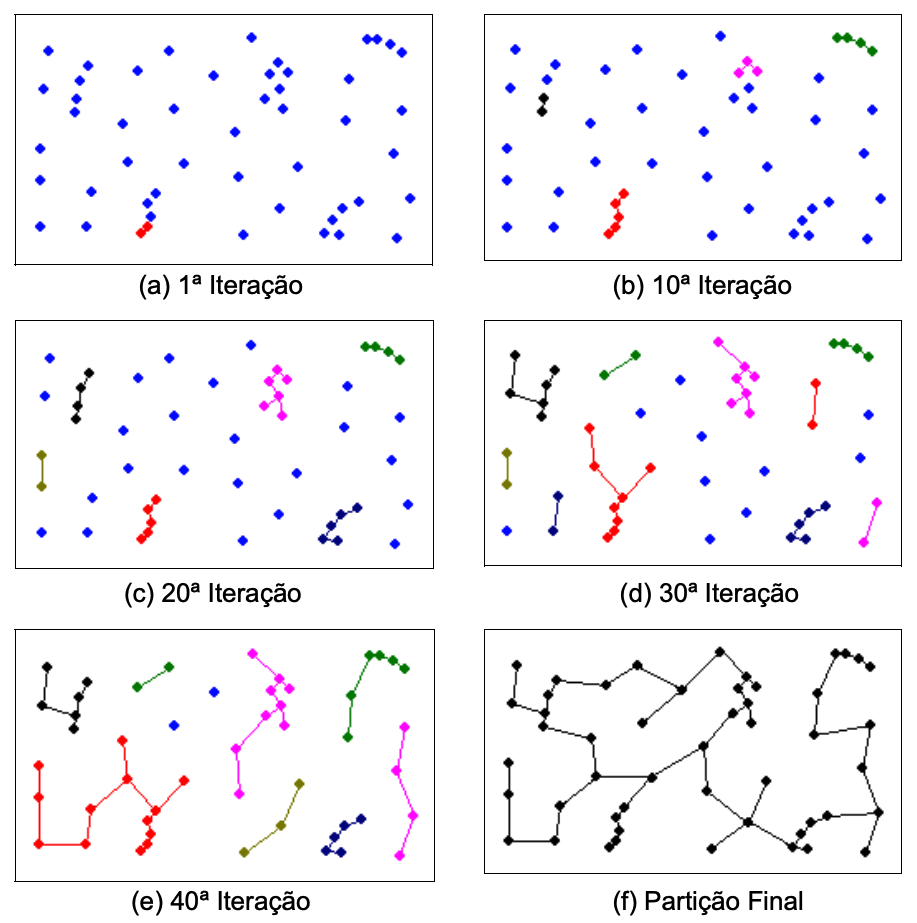
\includegraphics[width=14cm]{figuras/kruskal.png}
	}{
		\Fonte{\cite{joaoFrederico}}
	}
\end{figure}

\subsubsection{O algoritmo IGN}
 \label{sub:ign}
O IGN (Identificador de Grupos Naturais) \cite{ign} é baseado na construção de Árvore Geradora Mínima (AGM) sobre os dados do conjunto a classificar. Uma árvore geradora de um grafo conexo ${G = (V, E)}$ é uma estrutura em árvore ${T}$ que é um sub-grafo de ${G}$ e contém todos os vértices de ${G}$. Além disso, cada aresta ${e}$ possui um peso ${p(e)}$. Denomina-se peso de uma árvore geradora ${T=(V,E_T)}$ de ${G}$ a soma dos pesos das arestas ${E_T}$. Se um grafo é desconexo, não se pode identificar nenhuma árvore geradora. Mas pode-se identificar no mínimo uma floresta de árvores geradoras, uma para cada componente do grafo. Uma árvore geradora mínima é a árvore geradora de ${G}$ que possui peso mínimo dentre todas as árvores geradoras de ${G}$.
Este método é conceitualmente distinto dos demais, pois estabelece uma relação entre a construção da árvore hierárquica (árvore geradora mínima - AGM) e, de trás para frente, acompanhando a retirada dos elos (ligações entre classes) da árvore, o método evolui buscando a maior tangente da função de decaimento formada pelo custo de retirada das ligações da AGM.

O procedimento para identificar os grupos naturais para encontrar a melhor quantidade pode ser descrito a seguir:
 \begin{enumerate}
\item Executar o algoritmo de Kruskal guardando os custos dos grupos gerados. Iniciando de ${n}$ grupos até 1;
\item Encontrar o módulo da diferença entre o custo de cada iteração com os custos dos seus dois sucessores;
\item Selecionar a menor diferença entre o custo/valor da maior tangente obtido a cada iteração do passo anterior com o seu predecessor;
\item Retornar a composição das árvores do melhor resultado respeitando o parâmetro de quantidade mínima de elementos para se constituir um grupo.
\end{enumerate}

A complexidade do método IGN é ${O(n^2 log n)}$, onde ${n}$ é o número de indivíduos da base de dados. Após a execução do algoritmo de Kruskal, inicia os cortes nas árvores para as buscas dos grupos.
Algumas características desse método são:
\begin{itemize}
\item Apresenta bons resultados em qualquer métrica;
\item É sensível à presença de \emph{outliers} em situações muito específicas. Nestes casos pode apresentar resultados insatisfatórios quando houver proximidade de \emph{outliers} entre grupos naturalmente formados, confundindo os grupos naturais pela existência de "indivíduos pontes" (que surgem em função das dimensões de afastamento entre grupos inerentes);
\item Se há uma separação definida (um corte), o método é exato, ou seja, sempre encontrará os grupos naturais. Se a separação não existe, o método pode falhar;
\item Diferentemente dos demais, o número de grupos naturais e sua composição é obtida automaticamente no processo;
\item Usa o dendrograma de forma invertida para definir o ponto de corte (corte transversal no dendrograma), baseado na função monótona decrescente gerada pela função de custo de retirada das arestas da AGM (da maior para a menor) formada entre os indivíduos do processo de agrupamento.
\end{itemize}

Para facilitar as tarefas de análise multivariada, \cite{ign} desenvolveram o sistema SCLUSTER \cite{scluster}. Este \textit{software} é utilizado no exemplo seguinte apresentado em \cite{devillez}, onde um conjunto observado contém 236 pontos com duas variáveis, como exibe a figura \ref{fig:ignExemplo}. O resultado é a formação de quatro grupos, onde o primeiro possui 47 pontos, o segundo e o terceiro com 57, e o quarto com 41, além de 34 pontos do tipo \textit{outliers}.

\begin{figure}[!ht]
	\centering
	\Caption{\label{fig:ignExemplo} IGN - Grupo de dados com 4 grupos}	
	\UECEfig{}{
		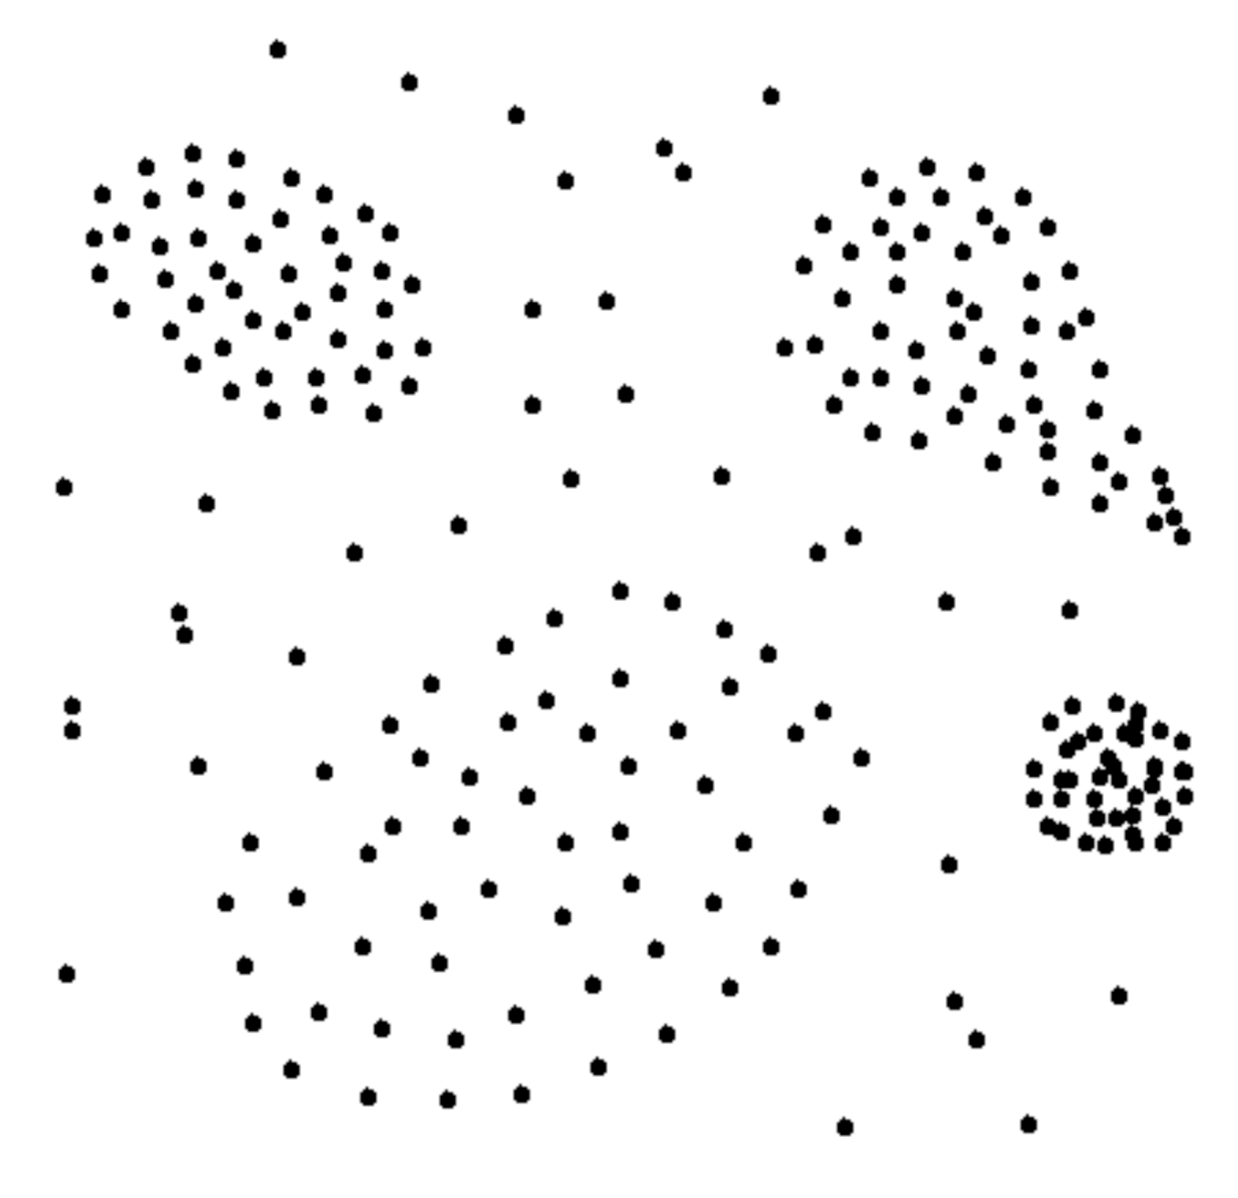
\includegraphics[width=10cm]{figuras/ignExemplo.png}
	}{
		\Fonte{\cite{joaoFrederico}}
	}
\end{figure}

Pode-se observar que os grupos foram identificados ao executar o algoritmo IGN separando os 236 pontos em quatro grupos, como mostrado na tabela \ref{tab:ignTabela} e figura \ref{fig:ignExemploResultado}.

\begin{table}[!ht]	
	\centering
	\Caption{\label{tab:ignTabela} IGN - Resultado para 4 grupos}
	\UECEtab{}{
		\begin{tabular}{|l|l|l|l|l|l|l|}
			\toprule
	    		Grupo & Grupo 01 & Grupo 02 & Grupo 03 & Grupo 04 & \textit{Outlier} & Total \\
			\midrule \midrule
				\begin{tabular}[c]{@{}l@{}}Pontos esperados por \\ grupo\end{tabular} & 47 & 57 & 57 & 41 & 34 & 236 \\
				\begin{tabular}[c]{@{}l@{}}Pontos alocados ao \\ grupo\end{tabular} & 47 & 57 & 57 & 41 & 34 & 236 \\
				\begin{tabular}[c]{@{}l@{}}Pontos alocados ao \\ grupo conforme o esperado\end{tabular} & 47 & 57 & 57 & 41 & 34 & 236 \\
				\begin{tabular}[c]{@{}l@{}}Pontos alocados ao \\ grupo diferente do esperado\end{tabular} & 0 & 0 & 0 & 0 & 0 & 0 \\
			\bottomrule
		\end{tabular}
	}{
		\Fonte{\cite{joaoFrederico}}
    }
\end{table}

\begin{figure}[!ht]
	\centering
	\Caption{\label{fig:ignExemploResultado} IGN - Agrupamento para 4 grupos}	
	\UECEfig{}{
		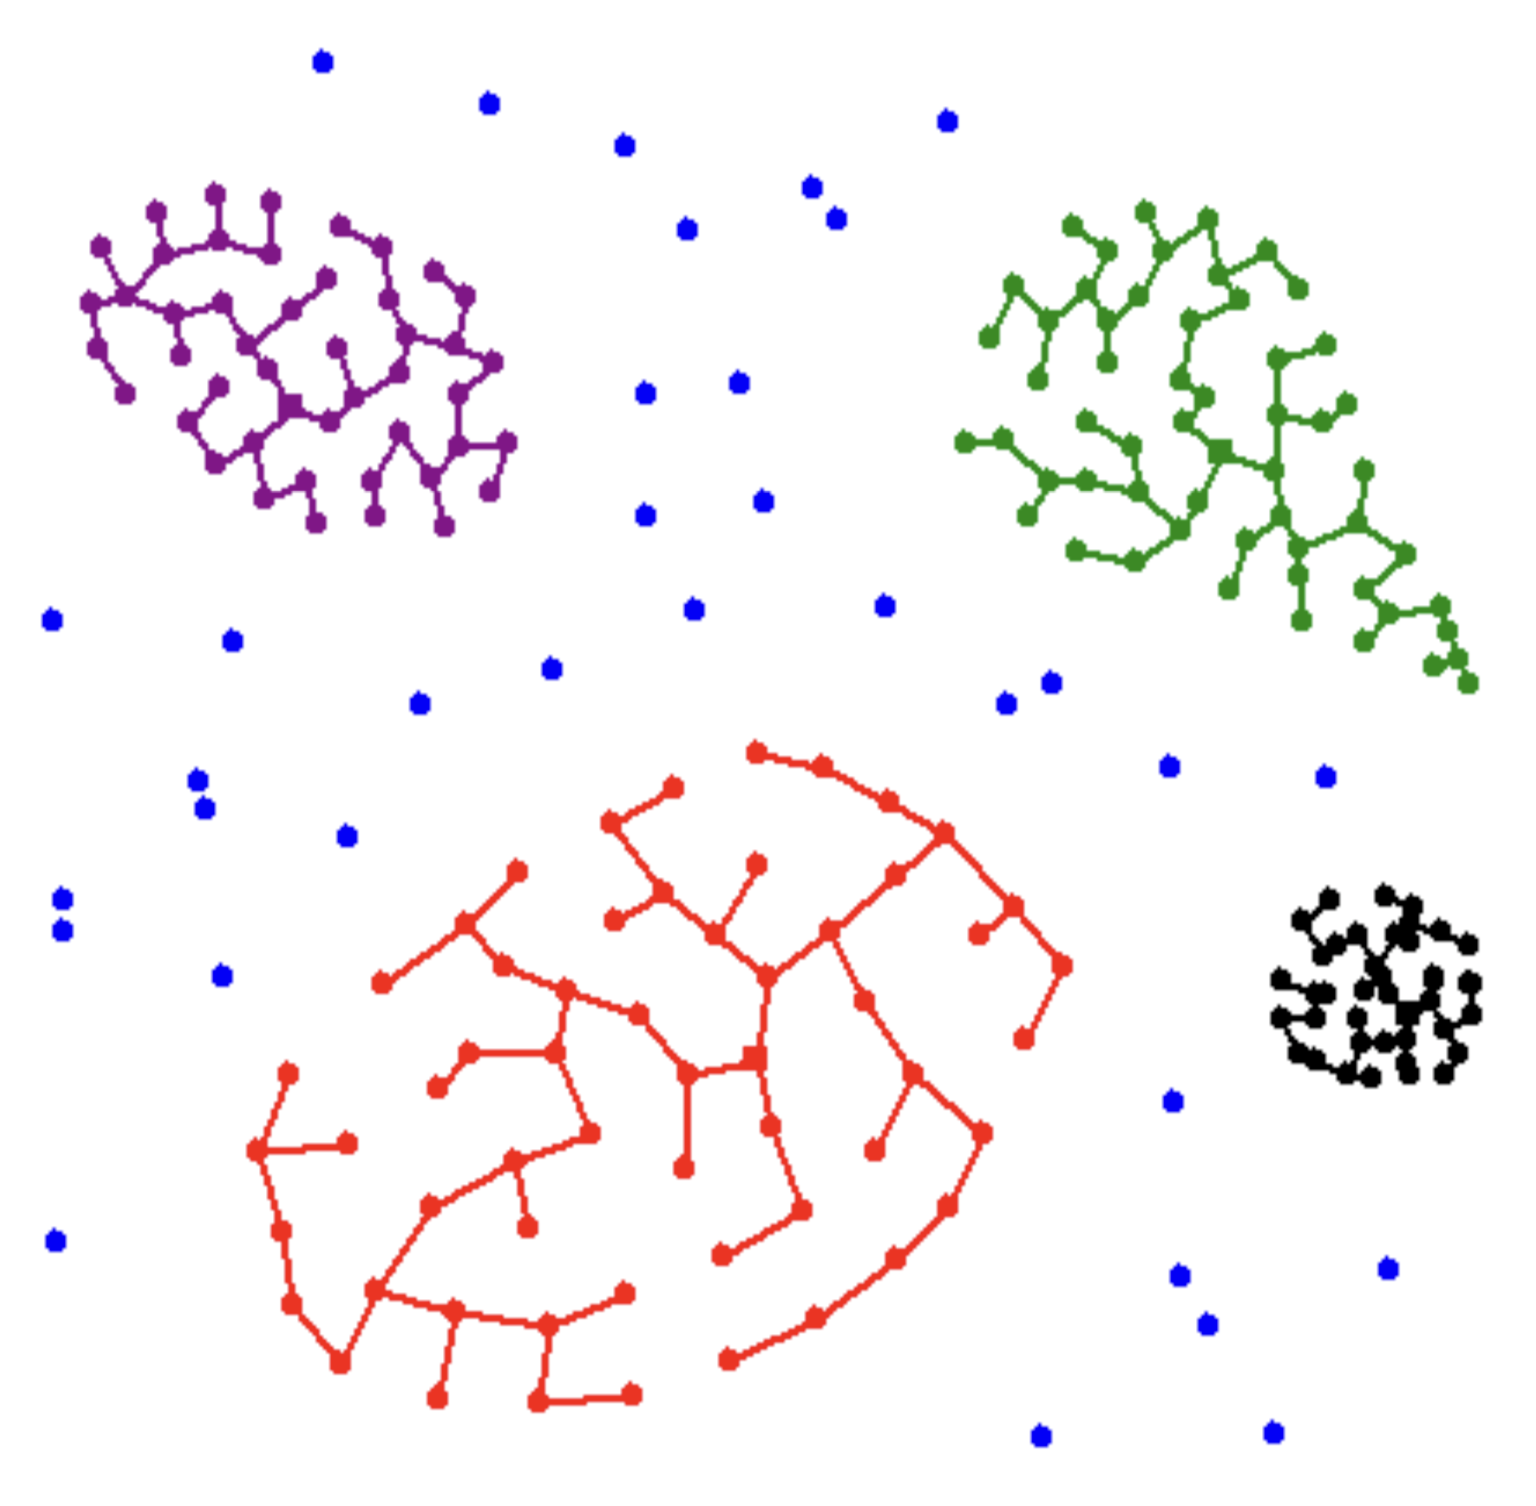
\includegraphics[width=10cm]{figuras/ignExemploResultado.png}
	}{
		\Fonte{\cite{joaoFrederico}}
	}
\end{figure}


\subsection{Métodos baseados em estrutura de grade}
Enquanto que os outros métodos de agrupamento discutidos são orientados aos dados, os métodos baseados em grade são orientados ao espaço. Essencialmente, o espaço é dividido em células retangulares, representadas por uma estrutura de grade hierárquica.

\subsubsection{O algoritmo STING}
\cite{Wang1997} propuseram um método de agrupamento baseado em grade, STING (\emph{STatistical INformation Grid} - Informação estatística baseada em grade), para agrupar bancos de dados espaciais e facilitar consultas orientadas à região. Esse algoritmo se baseia na construção de diversas camadas de grade, onde células de uma camada mais alta são subdivididas para a criação de células nas camadas mais baixas, como mostra a figura \ref{fig:sting}.

\begin{figure}[!ht]
	\centering	
	\Caption{\label{fig:sting} Algoritmo STING: subdivisão de células e construção de árvores}	
	\UECEfig{}{
		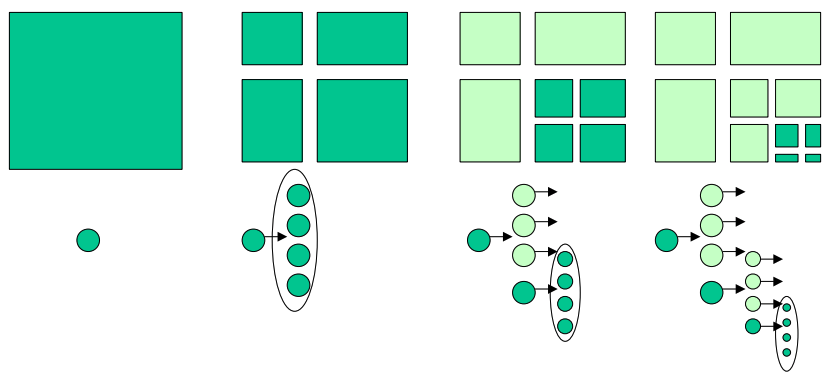
\includegraphics[width=8cm]{figuras/sting.png}
	}{
		\Fonte{\cite{Berkhin2002}}
	}
\end{figure}

O desempenho de STING depende da granularidade do nível mais baixo da estrutura de grade e o resultado dos
grupos são limitados, pois só crescem na horizontal ou vertical e sofrem para buscar grupos de formatos complexos.

Os resultados produzidos pelo STING se aproximam do agrupamento produzido pelo
DBSCAN à medida que a granularidade da estrutura de grade se aproxima de 0, podendo
também ser considerado como um método baseado em densidade, descrito a seguir.
Uma das vantagens do STING é a complexidade linear de tempo em relação ao número de objetos a serem agrupados.

\subsection{Métodos baseados em densidade}
Nesta classe de algoritmos a idéia principal é manter os grupos em crescimento, desde que sua densidade esteja acima de um certo limite. A vantagem dos algoritmos baseados em densidade, em comparação aos algoritmos de particionamento baseados em distância, é que eles podem detectar grupos de forma arbitrária. Isso também fornece uma proteção natural contra \textit{outliers}. Por outro lado, os algoritmos baseados na distância entre indivíduos detectam apenas aglomerados de forma convexa.

Os agrupamentos baseados em densidade analisam a quantidade de elementos dentro de uma vizinhança de acordo com determinados parâmetros. A ideia-chave é que, para cada instância de um grupo, a vizinhança de um determinado raio deve conter pelo menos um número mínimo de instâncias.

A possibilidade de encontrar agrupamentos de forma eventual e o fato de não precisar da definição do número de agrupamentos \cite{yip2005} como parâmetro inicial são as principais vantagens dos métodos baseados em densidade. Entretanto, alguns algoritmos podem exigir a definição de outros parâmetros, como o caso do algoritmo DBSCAN \cite{ESTER1996} abordado na próxima seção.

\subsubsection{Método DBSCAN}
\label{dbscan}
% TODO DBSCAN KDD96-037
% TODO O metodo dbscan https://www.maxwell.vrac.puc-rio.br/24787/24787_6.PDF

Este método calcula a densidade de uma região contando quantos objetos nela existem seguindo uma determinada métrica (p.ex., euclidiana ou manhattan). É um método efetivo para identificar grupos de formato arbitrário e de diferentes tamanhos, separar os ruídos dos dados, requer apenas um parâmetro de entrada, ajuda o usuário na determinação de um valor apropriado para ele e ajuda a detectar grupos e seus arranjos dentro do espaço de dados, sem qualquer informação preliminar sobre os grupos.
\cite{ESTER1996}  indicam que a noção de agrupamentos e o algoritmo DBSCAN se aplicam para espaços euclidianos de duas e três dimensões, como para qualquer espaço característico de alta dimensão. O método DBSCAN é aplicável a qualquer base de dados contendo dados de um espaço métrico, isto é, bases de dados com uma função de distância para pares de objetos. Finalmente, o DBSCAN é eficiente mesmo para grandes bancos de dados espaciais.

Para entender o método é necessário conhecer alguns conceitos básicos que são por ele utilizados: 

\begin{enumerate}
	\item Vizinhança: Determinada pela função de distância, que pode ser distância euclidiana ou distância manhattan, para dois pontos ${p}$ e ${q}$, dado por ${dist(p,q)}$.
	\item Eps: raio ao redor de um ponto. 
	\item Eps-vizinhança: a vizinhança de um ponto ${p}$ com raio Eps, dado por ${N_{Eps}(p)}$, é definido por ${N_{Eps}(p) = \big\{ q \in D | dist(p, q)  \leqslant Eps\big\} }$. Na figura \ref{fig:epsViz} abaixo os círculos representam respectivamente a vizinhança Eps dos pontos ${q}$ e ${p}$.
	\item Ponto Central: Se o Eps-vizinhança de um ponto ${p}$ contém ao menos um número mínimo, MinPts, de pontos, então o ponto ${p}$ é chamado de ponto central.
	Por exemplo, na figura \ref{fig:epsViz}, se for adotado MinPts = 4, ${p}$ é um ponto central e os demais não são pontos centrais.
	\item Ponto de Borda: Se a Eps-vizinhança de um ponto ${p}$ contém algum ponto central e menos que MinPts então o ponto ${p}$ é chamado de ponto de borda. Na figura  \ref{fig:epsViz}, ${q}$, ${r}$ e ${s}$ são pontos de borda.
	\item Diretamente alcançável: um ponto ${p}$ é alcançável se ele está no Eps-vizinhança de ${q}$ e este é um ponto central.
	\item Maximalidade: um ponto ${p}$ é alcançável se existe uma cadeia de pontos que os liga, respeitando Eps e MinPts.
	\item Conectividade: Um ponto ${p}$ está conectado a um outro ${q}$ se existe um objeto ${o}$ tal que tanto ${p}$ quanto ${q}$ são alcançáveis a partir de ${o}$, com respeito a Eps e MinPts. Logo é uma relação simétrica.
	\item Cluster: Seja D uma base de dados, um grupo C é um subconjunto não vazio de D, respeitando Eps e MinPts, onde:
		\subitem ${\forall}$ ${p}$, ${q}$ se ${q}$ ${\in}$ C e ${p}$ é alcançável a partir de ${q}$.
		\subitem ${\forall}$ ${p}$, ${q}$ ${\in}$ C ${p}$ está conectado por densidade a ${q}$.
\end{enumerate}

\begin{figure}[!ht]
	\centering
	\Caption{\label{fig:epsViz} Eps-vizinhança de ${q}$ e Eps-vizinhança de ${p}$}	
	\UECEfig{}{
		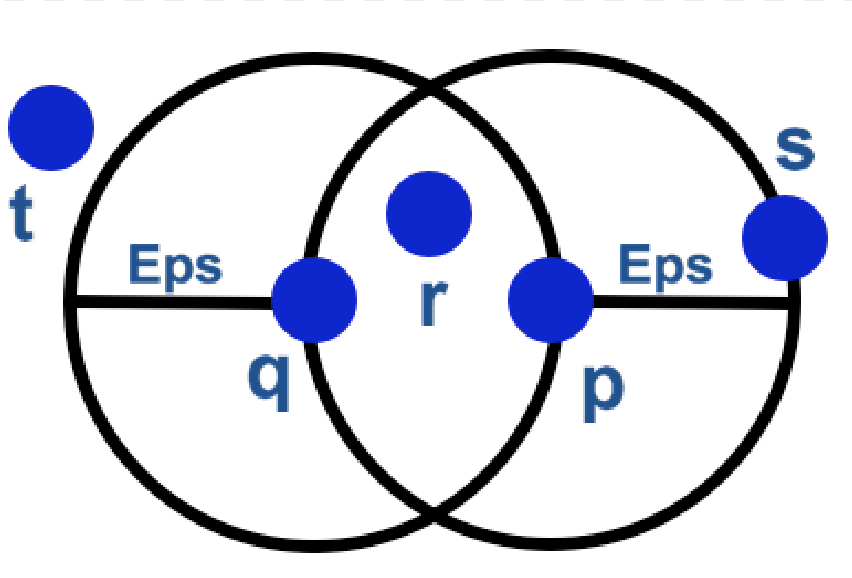
\includegraphics[width=8cm]{figuras/epsViz.png}
	}{
		\Fonte{Elaborado pelo autor}
	}
\end{figure}

O procedimento para encontrar um agrupamento é baseado no fato de que um grupo é inequivocamente determinado por qualquer de seus centros \cite{ESTER1998}. 

O DBSCAN pode utilizar a estrutura de dados R*-tree para obter um melhor desempenho, mesmo assim  a complexidade média do tempo de execução do DBSCAN será ${O (N logN)}$, onde ${N}$ é o número de objetos da base de dados, \cite{Sheikholeslami1998}.

\subsubsubsection{Algoritmo DBSCAN}

As etapas envolvidas neste algoritmo são as seguintes:

\begin{enumerate}
	\item Selecionar um ponto arbitrário ${p}$;
	\item Recuperar todos os pontos que são alcançáveis por densidade a partir do ponto ${p}$;
	\item Se ${p}$ é um ponto central, um grupo é formado;
	\item Se ${p}$ é um ponto de borda, nenhum ponto é alcançável por densidade a partir de ${p}$ e DBSCAN visita o próximo ponto do banco de dados;
	\item Continuar o processo até que todos os pontos tenham sido processados.
\end{enumerate}

% ver https://www.maxwell.vrac.puc-rio.br/24787/24787_6.PDF

\begin{algorithm}[!ht]
	\SetSpacedAlgorithm
	\caption{\label{alg:algoritmo_dbscan}Algoritmo DBScan}
	\Entrada{D, Eps1, MinPts, Delta, Epsilon}
	\Saida{C}
	\Inicio{
			\Para{i = 0 até n}{
				\Se{${o_i}$ nao foi visitado}{
					marcar ${o_i}$ como visitado\;
					Vizinhos = BuscarVizinhos(${o_i}$)\;
					\Se {|Vizinhos| < MinPts}{
						MarcarRuido(${o_i}$)\;
					}
				    \Senao{
				    	C = próximo Cluster\;
				    	adicionar ${o_i}$ ao cluster C\;
				    	expandirCluster(${o_i}$, C, Vizinhos)\;
				    }
				}
			}
	}
\end{algorithm}
\begin{algorithm}[!ht]
	\SetSpacedAlgorithm
	\caption{\label{alg:algoritmo_dbscan_exp}Algoritmo DBScan - Expandir Cluster}
	\Entrada{Vizinhos, C, MinPts}
	\Inicio{
			\Para{i = 0 até número de Vizinhos}{
				${p}$ = ${Vizinhos_{(i)}}$\;
				\Se {${p}$ ainda não foi visitado}{
					marcar ${p}$ como visitado\;
					Vizinhos2 = BuscarVizinhos(p)\;
					
					\Se {Vizinhos2 ${\geqslant}$ MinPts}{
						Vizinhos = Vizinhos ${\cup}$ Vizinhos2\;
					}
				}
				\Se{${p}$ não está em nenhum cluster}{
					adicionar ${p}$ ao cluster C\;
				}
				
			}
	}
\end{algorithm}
\pagebreak
As figuras \ref{fig:dbscanStep1}, \ref{fig:dbscanStep2} e \ref{fig:dbscanStep3} ilustram os passos da resolução do algoritmo DBSCAN.

\begin{figure}[!ht]
	\centering
	\Caption{\label{fig:dbscanStep1} DBSCAN - Identificação dos vizinhos dentro de um raio definido}	
	\UECEfig{}{
		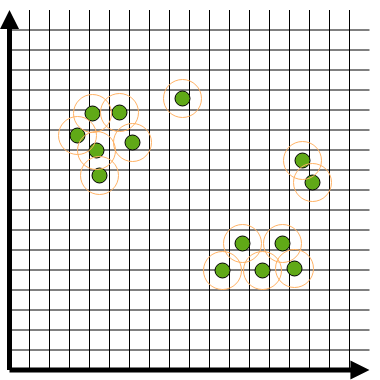
\includegraphics[width=9cm]{figuras/dbscanStep1.png}
	}{
		\Fonte{Elaborado pelo autor}
	}
\end{figure}

\begin{figure}[!ht]
	\centering
	\Caption{\label{fig:dbscanStep2} DBSCAN - Pontos que estejam dentro do raio de outro ponto estão no mesmo grupo}
	\UECEfig{}{
		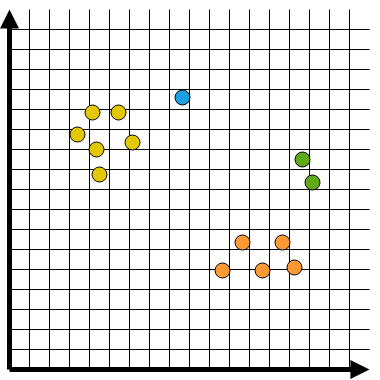
\includegraphics[width=9cm]{figuras/dbscanStep2.png}
	}{
		\Fonte{Elaborado pelo autor}
	}
\end{figure}

\begin{figure}[!ht]
	\centering
	\Caption{\label{fig:dbscanStep3} DBSCAN - Identificação dos \textit{outliers}}	
	\UECEfig{}{
		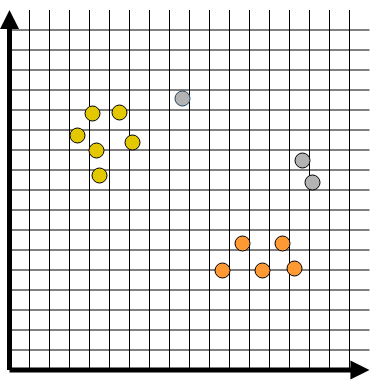
\includegraphics[width=10cm]{figuras/dbscanStep3.png}
	}{
		\Fonte{Elaborado pelo autor}
	}
\end{figure}

\subsection{Processo de detecção de \textit{outliers}}

Um \textit{outlier} é um objeto que desvia de um padrão do conjunto de dados ao qual ele pertence. Segundo \cite{Barnett1978Outliers}, é uma observação (ou um conjunto de observações) que parece ser inconsistente com o restante daquele conjunto de dados. Ele descreve as causas de ocorrência de \textit{outliers} como: são objetos que pertencem a população; erro de medição na coleta de dados; erros de execução ao adquirir dados de amostragem de mais de uma população.

Em processos de agrupamento é muito importante a detecção dos \textit{outliers}, uma vez que estes objetos podem deturpar o processo de classificação de forma muito danosa. Deve-se pois considerar também que vários dos métodos de agrupamentos naturais servem também como bons detectores de \textit{outliers}, no entanto as características destes indivíduos podem ser muito relevantes para a separação completa dos demais que têm similaridades características de cada um dos grupos a que pertencem.

%Outlier x Ruídos
Uma questão a se considerar é a diferença entre o significado de \textit{outlier} e ruído. Enquanto ruído refere-se à modificação de valores originais, os \textit{outliers} contêm informações importantes para a descricão do conjunto de dados \cite{chandola2009}. Ruído é uma anomalia indesejada no dado causada por imprecisão nos atributos de entrada, erro ao rotular os dados ou até por atributos de dados que foram excluídos, mas afetam a rotulação \cite{alpaydin2010}.

A detecção de \textit{outliers} refere-se ao problema de encontrar padrões que exibem um comportamento diferenciado em relação à maioria dos dados \cite{chandola2009}. Caracterizar o processo de detecção de ruídos e \textit{outliers} é muito importante, pois permite a redução de prejuízos e uma melhor análise dos dados. As técnicas de detecção \textit{outlier} têm sido aplicadas a um grande número de aplicações tais como: detecção de fraudes, processamento de imagens, detecção de intrusão, medicina e detecção de dados rotulados incorretamente.

\subsubsection{Técnicas de detecção de \textit{outliers}}
As técnicas de detecção de \textit{outliers} podem ser aplicadas em detecção de padrões raros, remoção de ruídos, detecção de padrões ainda não observados, etc. Deve-se considerar a complexidade computacional dada a grandes quantidades de dados disponíveis para manipulação. Alguns fatores são importantes para classificar as técnicas de detecção de \textit{outliers}: a natureza dos dados, o tipo de \textit{outlier}, a disponibilidade dos rótulos, a utilização de parâmetros, a manipulação de grande volume de dados, etc. A seguir, algumas das técnicas de detecção de \textit{outliers}.

\subsubsubsection{Técnicas estatísticas}
As técnicas estatísticas desenvolvem um modelo estatístico (geralmente para um comportamento normal) aos dados fornecidos e, em seguida, aplicam um teste de inferência estatística para determinar se um determinado dado pertence ou não a esse modelo. Dados com baixa probabilidade de pertencerem ao modelo estatístico são declaradas como \textit{outlier} \cite{chandola2009}.

\subsubsubsection{Técnicas baseadas em distância}
Técnicas baseadas em distância são aquelas que variam a forma de computar a distância de um objeto em relação aos vizinhos mais próximos. A distância pode ser medida por meio da distância de Manhattan ou Euclidiana e a escolha do valor não depende do conjunto de dados. Existem técnicas que se baseiam no cálculo da densidade de objetos para identificar \textit{outliers}. O funcionamento segue duas etapas: para cada dado a vizinhança é computada usando uma medida de distância ou de similaridade entre dois dados. Na segunda etapa, os vizinhos são analisados para determinar se o dado é normal ou \textit{outlier}.

\subsubsubsection{Técnicas baseadas em agrupamento de dados}
Técnicas baseadas em agrupamento levam em consideração que dados normais pertencem a grupos grandes e densos, enquanto objetos de dados \textit{outliers} não se enquadram em nenhum grupo. O principal objetivo dos algoritmos de agrupamento de dados é na identificação de grupos, e por isso é necessário estabelecer algum critério para diferenciar um dado normal de um \textit{outlier}.

O algoritmo de BIRCH \cite{Zhang1996} mencionado na seção \ref{sub:birch}, considera como \textit{outliers} as entradas de baixa densidade presentes nos nós folhas da AC-árvore.

Estas técnicas podem ser divididas em semi-supervisionadas e não-supervisionadas. As técnicas semi-supervisionadas normalmente usam dados normais para gerar grupos que representam o comportamento normal dos dados, um objeto novo de teste é alocado a um grupo, se não estiver próximo de nenhum é categorizado como \textit{outlier}. Já as técnicas não-supervisionadas usam um algoritmo conhecido de agrupamento para agrupar os dados e analisam cada instância com relação aos grupos formados.

\section{Agrupamentos Dinâmicos}
Um agrupamento dinâmico é definido como sendo um conjunto de indivíduos de alta similaridade que se mantêm unido ao longo do tempo, caracterizado por um certo número de indivíduos que mantêm a identidade do grupo. O processo de classificação de agrupamentos dinâmicos é a metodologia que identifica tais grupos que se constroem e se desfazem no tempo, tal metodologia identifica classes naturais e ao mesmo tempo as relaciona a outras classes em similaridade que ocorrem antes e depois delas no tempo. Tal relação precisa ser bem estabelecida e consistente para que se perceba os movimentos evolutivos no tempo.

Várias formas diferentes de tipos de dados espaço-temporais estão disponíveis em aplicativos reais. Embora todos compartilhem a disponibilidade de algum tipo de aspecto espacial e temporal, a extensão dessas informações e a maneira como elas são relacionadas podem se combinar com vários tipos diferentes de objetos de dados \cite{maimon:2005}. Com base em duas dimensões, é dada uma possível classificação destes tipos de dados:

\begin{itemize}
	\item a dimensão temporal descreve em que medida a evolução do objeto é capturada pelos dados. O caso mais básico consiste em objetos que não evoluem, onde apenas um \textit{snapshot} estático de cada objeto está disponível. Em contextos um pouco mais complexos, cada objeto pode alterar seu status, mas apenas seu valor mais recente é conhecido (um \textit{snapshot} atualizado), portanto, sem qualquer conhecimento sobre seu histórico passado. No caso extremo é onde o histórico completo do objeto é mantido, formando assim uma série temporal do status que ele percorreu;

	\item a dimensão espacial descreve se os objetos considerados estão associados a um local fixo (por exemplo, as informações coletadas por sensores fixados no solo) ou podem se mover, ou seja, sua localização é dinâmica e pode mudar no tempo.
\end{itemize}

\subsection{Método ST-DBSCAN}
\label{stdbscan}

% Comentar um bloco de código: \iffalse \fi
Para agrupar os pontos levando em conta o fator tempo é necessário uma alteração no algoritmo DBSCAN \cite{ESTER1998}, e com isso detectar os grupos em relação ao tempo. Esse algoritmo usa apenas um parâmetro de distância Eps para medir a similaridade de dados espaciais com uma dimensão. A fim de suportar dados espaciais bidimensionais, o ST-DBSCAN \cite{Birant2007STDBSCANAA} usa duas métricas de distância, Eps1 e Eps2, para definir a similaridade por uma conjunção de dois testes de densidade.
O algoritmo ST-DBSCAN é construído modificando o algoritmo DBSCAN. Em contraste com o algoritmo de agrupamento baseado em densidade existente, o algoritmo ST-DBSCAN tem a capacidade de descobrir agrupamentos de acordo com valores não espaciais, espaciais e temporais dos objetos. As três modificações feitas no algoritmo DBSCAN são as seguintes:
\begin{itemize}
\item Permitir o algoritmo ST-DBSCAN descobrir grupos em dados espaciais-temporais.
\item Introdução do fator de densidade atribuído a cada grupo, que é o seu grau de densidade, para encontrar objetos de ruído quando existem grupos de diferentes densidades.
\item A terceira modificação fornece uma comparação do valor médio de um grupo com o novo valor resultante. Necessária para resolver os conflitos em pontos de borda.
\end{itemize}

O algoritmo DBSCAN não é satisfatório quando existem agrupamentos de diferentes densidades. Para superar esse problema,  o ST-DBSCAN atribui a cada grupo um fator de densidade, que é o grau da densidade do grupo.
A função DensityDistance é dada por:

${DensityDistance = \frac{DensityDistanceMax}{DensityDistanceMin}}$
\linebreak
onde DensityDistanceMax de um objeto ${p}$ denota a distância máxima entre o objeto ${p}$ e seus vizinhos dentro do raio Eps. Da mesma forma, DensityDistanceMin de um objeto ${p}$ denota a distância mínima entre o objeto ${p}$ e seus vizinhos dentro do raio Eps.

${DensityDistanceMax(p) = max\big\{ dist(p, q) | q \in D \wedge dist(p, q)  \leqslant Eps\big\} }$

${DensityDistanceMin(p) = min\big\{ dist(p, q) | q \in D \wedge dist(p, q)  \leqslant Eps\big\} }$
\linebreak

O fator de densidade de um grupo ${C}$ é dado por:

${DensityFactor(C) = 1\big/\left [   \frac{\sum_{p\in C}DensityDistance(p)}{|C|} \right ]}$
\linebreak

Com esse fator é possível evitar problemas de agrupamentos com grande variação de densidade, onde os grupos são pequenos e muito densos ou grandes e pouco densos.

\subsubsection{Algoritmo ST-DBSCAN}
Uma grande diferença entre o DBSCAN e o ST-DBSCAN é a utilização de um segundo parâmetro EPS, onde é usado para medir a similaridade de valores não espaciais. Nesta pesquisa usa-se o tempo como EPS de valor não espacial. Para dois pontos serem considerados vizinhos eles devem respeitar os limites de espaço e tempo parametrizados por EPS1 e EPS2 \cite{Birant2007STDBSCANAA}.

\begin{enumerate}
	\item O algoritmo começa com o primeiro ponto ${p}$ no banco de dados D.
	\item Este ponto ${p}$ é processado de acordo com o algoritmo DBSCAN e o próximo ponto é tomado.
	\item A função BuscarVizinhos(p, Ep1, Ep2) recupera todos os pontos que tem uma distância menor que Eps1 e Eps2 para o ponto ${p}$. Se os pontos recuperados não podem ser alcançados o ponto é atribuído como ruído, onde o ponto selecionado não tem vizinhos suficientes para ser armazenado em grupo.
	\item Os pontos marcados como ruído podem ser alterados posteriormente, se não forem diretamente alcançáveis pela densidade, mas eles são alcançáveis por densidade de algum outro ponto do banco de dados. Isso acontece para pontos de borda de um grupo.
	\item Se o ponto selecionado tiver vizinhos suficientes dentro das distâncias Eps1 e Eps2 - se for um ponto central, então um novo grupo será construído.
	\item Todos os vizinhos diretamente atingíveis por densidade desse ponto central também são incluídos.
	\item O algoritmo reúne iterativamente pontos acessíveis por densidade a partir desse ponto central usando uma pilha.
	\item Se o objeto não estiver marcado como ruído ou não estiver em um grupo e a diferença entre o valor médio do grupo e o novo valor é menor do que o valor limite para incluir em um grupo, ${\Delta E}$, ele é colocado no grupo atual.
	\item Se dois grupos ${C_1}$ e ${C_2}$ estão muito próximos um do outro, um ponto ${p}$ pode pertencer a ambos ${C_1}$ e ${C_2}$. Então o ponto ${p}$ é atribuído ao grupo que foi descoberto primeiro.
	\item Depois de processar o ponto selecionado, o algoritmo seleciona o próximo ponto em D e o algoritmo continua iterativamente até que todos os pontos tenham sido processados.
\end{enumerate}

\pagebreak
\begin{algorithm}[!ht]
	\SetSpacedAlgorithm
	\caption{\label{alg:algoritmo_stdbscan}Algoritmo ST-DBScan}
	\Entrada{D, Eps1, Eps2, MinPts, ${\Delta E}$}
	\Saida{C = (${C_1}$, ${C_2}$, ... ${C_k}$) Conjunto de clusters}
	\Inicio{
		\Para{i = 1 até n}{
			\Se {${o_i}$ não está no cluster}{
				Vizinhos = BuscarVizinhos(${o_i}$, Eps1, Eps2)\;
				\Se {|Vizinhos| < MinPts}{
					marcar ${p}$ como ruído\;
				}
			   \Senao{
			   		\Para{j = 1 até |Vizinhos|}{
			   			RotularPontos(${X_j}$)\;
			   			AdicionarPontosAoCluster(${X_j}$, ${C_i}$)\;
			   		}
		   		\Enqto{existir pontos na vizinhança de ${o_i}$}{
		   			pontoAtual = vizinho(${o_i}$)\;
		   			Vizinhos2 = BuscarVizinhos(pontoAtual, Eps1, Eps2)\;
		   			\Se{|Vizinhos2| >= MinPts}{
		   				\Para{ todo ${o_y}$}{
		   					\Se{(${\neg}$ehRuido(${o_y}$) ${\vee}$ ${\neg}$estaNumGrupo(${o_y}$)) ${\wedge}$ DensidadeMediaDoGrupo($C_i$) +${o_y}$ > ${\Delta E}$ }{
		   						AdicionarPontosAoCluster(${o_y}$, ${C_i}$)\;
		   					}
		   				}
		   			}
		   		}
		       }
			}
		}
	}
\end{algorithm}

Um exemplo do ST-DBSCAN é apresentado em \cite{st-twitter}, onde o Eps1 é definido como 70km, 85km e 100km, e MinPts como 5, 10 e 15. Já o Eps2 como 2 dias. Os resultados para os 9 conjuntos de parâmetros são mostrados na figura \ref{fig:st-twitter}, revelando claramente que um maior Eps e um menor MinPts correspondem a maiores grupos espaço-temporais. Na Figura \ref{fig:st-twitter}(a), duas regiões espaço-temporais são representadas por duas elipses pretas, denominadas STR1 e STR2.
Os parâmetros de cada conjunto são:
(a) Eps = 70, MinPts = 5; (b) Eps = 85, MinPts = 5; (c) Eps = 100, MinPts = 5; (d) Eps = 70, MinPts = 10; (e) Eps = 85, MinPts = 10; (f) Eps = 100, MinPts = 10; (g) Eps = 70, MinPts = 15; (h) Eps = 85, MinPts = 15; (i) Eps = 100, MinPts = 15. O Eps2 (2 dias) é o mesmo para todos os conjuntos.

\begin{figure}[!ht]
	\centering
	\Caption{\label{fig:st-twitter} ST-DBSCAN - Os clusters espaço-temporais descobertos}
	\UECEfig{}{
		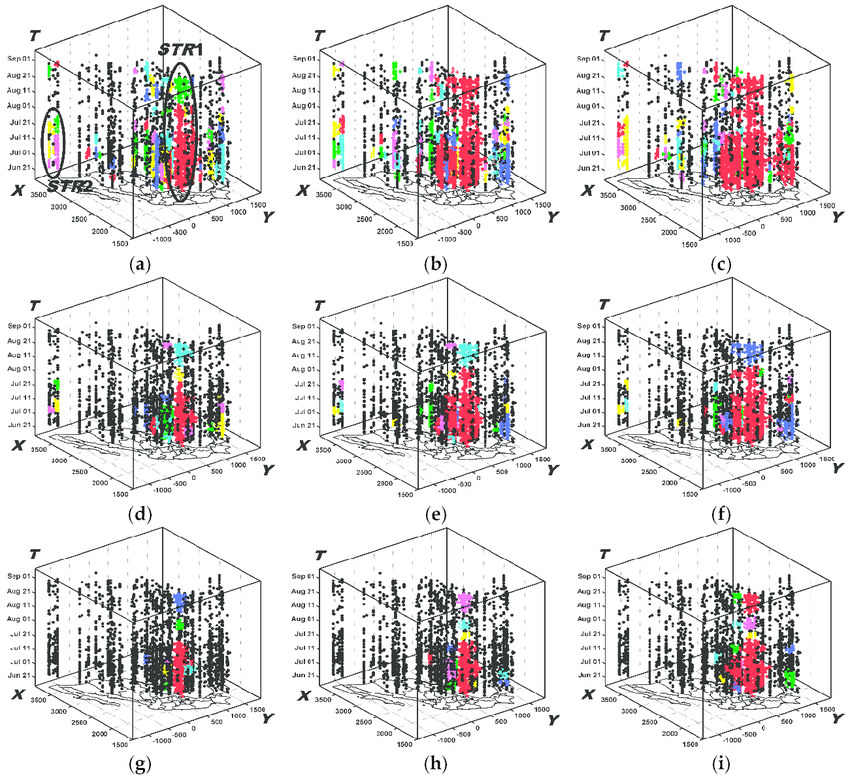
\includegraphics[width=16cm]{figuras/st-twitter.png}
	}{
		\Fonte{\cite{st-twitter}}
	}
\end{figure}

\subsection{Método ST-IGN}
\label{stign}
O método IGN dinâmico consiste da aplicação do método IGN estático \cite{simposioNeg2003} sobre cada uma das $n$ instâncias (estados) geradas a partir de um período (intervalo fixo de estados) definido pelo processo de identificação da dinâmica do comportamento dos objetos. O método rotula os grupos naturais encontrados na unidade de tempo $i$ com base na máxima densidade de objetos que se mantém no mesmo grupo após uma divisão e/ou aglomeração.

A seguir são listados os elementos e parâmetros necessários para aplicação do método:
\begin{itemize}
\item Objetos de Entrada definidos por estado;
\item Unidade de tempo estático (uma fotografia);
\item Período Dinâmico (intervalo interno da fotografia);
\item Ganho Estático (possibilidade de ganho de estados em períodos distintos).
\end{itemize}

Os indivíduos podem ser representados atráves de uma entrada de dados, que consiste de uma tabela com as seguintes características:

\begin{table}[!ht]
	\centering
	\Caption{\label{tab:label_da_tabela} IGN Dinâmico - Estrada de dados}
	\UECEtab{}{
		\begin{tabular}{c c c c c c c c}
			\toprule
	            & ${X_1}$ & ${X_2}$ & ${X_3}$ & ... & ${X_p}$ & ${X_t}$ &\\
	    	    ${I_{11}}$	&  &  &  &  &  &  & 1\\
	    	    ${I_{21}}$	&  &  &  &  &  &  & 1\\
	    	    . &  &  &  &  &  &  & .\\
	    	    . &  &  &  &  &  &  & .\\
	    	    . &  &  &  &  &  &  & .\\
	    	    ${I_{n1}}$	&  &  &  &  &  &  & 1\\
	    	    ${I_{12}}$	&  &  &  &  &  &  & 2\\
	    	    . &  &  &  &  &  &  & .\\
	    	    . &  &  &  &  &  &  & .\\
	    	    . &  &  &  &  &  &  & .\\
	    	    ${I_{n2}}$	&  &  &  &  &  &  & 2\\
	    	    ${I_{1m}}$	&  &  &  &  &  &  & m\\
	    	    . &  &  &  &  &  &  & .\\
	    	    . &  &  &  &  &  &  & .\\
	    	    . &  &  &  &  &  &  & .\\
	    	    ${I_{nm}}$	&  &  &  &  &  &  & m\\
			\bottomrule
		\end{tabular}
	}{
		\Fonte{Elaborado pelo autor}
    }
\end{table}

Onde, 

${I_{ik}}$, é o indivíduo do estado \textit{k};

${X_s}$, é o valor do atributo referente a variável \textit{s};

${X_t}$, é a variável que indica o estado \textit{t} a que pertence o indivíduo.

Sejam estão os seguintes parâmetros para avaliação de um movimento dinâmico:
\begin{itemize}
    \item NE - Número de estados;
    \item TPE - Tamanho do período estático. Quantidade de estados sequenciais a serem tomados, ${TPE \geqslant 1}$;
    \item TPD - Tamanho do período dinâmico. Toma os próximos TPE estados e elimina os TPE estados anteriores, ${TPD \geqslant 1}$;
    \item GD - Ganho dinâmico. Quantidade de estados ganhos ou perdidos entre dois períodos dinâmicos subsequentes, ${GD \geqslant 0}$;
    \item GN[k] - É o conjunto dos grupos naturais formados na iteração \textit{k};
    \item DATA[k] - É o conjunto formado pelos dados do período estático \textit{k}.
\end{itemize}

O algoritmo que define o método IGN Dinâmico pode ser escrito da seguinte forma:

\begin{algorithm}[!ht]
	\SetSpacedAlgorithm
	\caption{\label{alg:algoritmo_stign}Algoritmo ST-IGN}
	\Entrada{TPE, TPD, GD}
	\Saida{GN - Grupos Naturais}
	\Inicio{
	    i = TPE\;
	    k = 1\;
	    s = 0\;
	    \Enqto{${s \geqslant NE}$}{
    	    \Se {${s = 0}$} {
	            ${t_1 = 1}$\;
    	    }
    	    \Senao {
    	        ${t_1 = t_1 + TPD}$\;
    	    }
    	    ${t_2 = t_1 + TPE + GD - 1}$\;
    	    ${DATA[k] = \{ I_s, s = t_1, ..., t_2 \} }$\;
    	    IGN-Estatico(${DATA[k], GN[k]}$)\;
    	    AvaliarRotular(${GN[k]}$, ${GN[[k-1]}$)\;
    	    ${k = k + 1}$\;
	    }
	}
\end{algorithm}

O procedimento IGN-Estático retorna o agrupamento ${GN[k]}$ para os dados do período estático ${DATA[k]}$. Já o algoritmo AvaliarRotular, refaz a rotulação e caracterização do grupo ${GN[k]}$ com base na rotulação do agrupamento anterior ${GN[k - 1]}$, preservando ao máximo os elementos deste agrupamento no novo agrupamento.

A figura \ref{fig:ign_avaliar_rotular} apresenta o processo de rotulação do procedimento AvaliarRotular, para os grupos formados para dados do período ${k - 1}$ e \textit{k}. Sendo ${GN[k]}$ e ${GN[k - 1]}$, onde ${GN[k] \cap GN[k - 1] \neq \varnothing 
}$, a rotulação de ${GN[k - 1]}$ será mantida em ${GN[k]}$ naqueles grupos que têm a maior quantidade de elementos em relação ao seu gerador em ${GN[k - 1]}$. Caso não haja interseções entre grupos nos períodos subsequentes distintos, novos rótulos serão atribuídos a estes grupos.

\begin{figure}[!ht]
	\centering
	\Caption{\label{fig:ign_avaliar_rotular} Procedimento AvaliarRotular e evolução do IGN-Dinâmico para 3 períodos estáticos}	
	\UECEfig{}{
		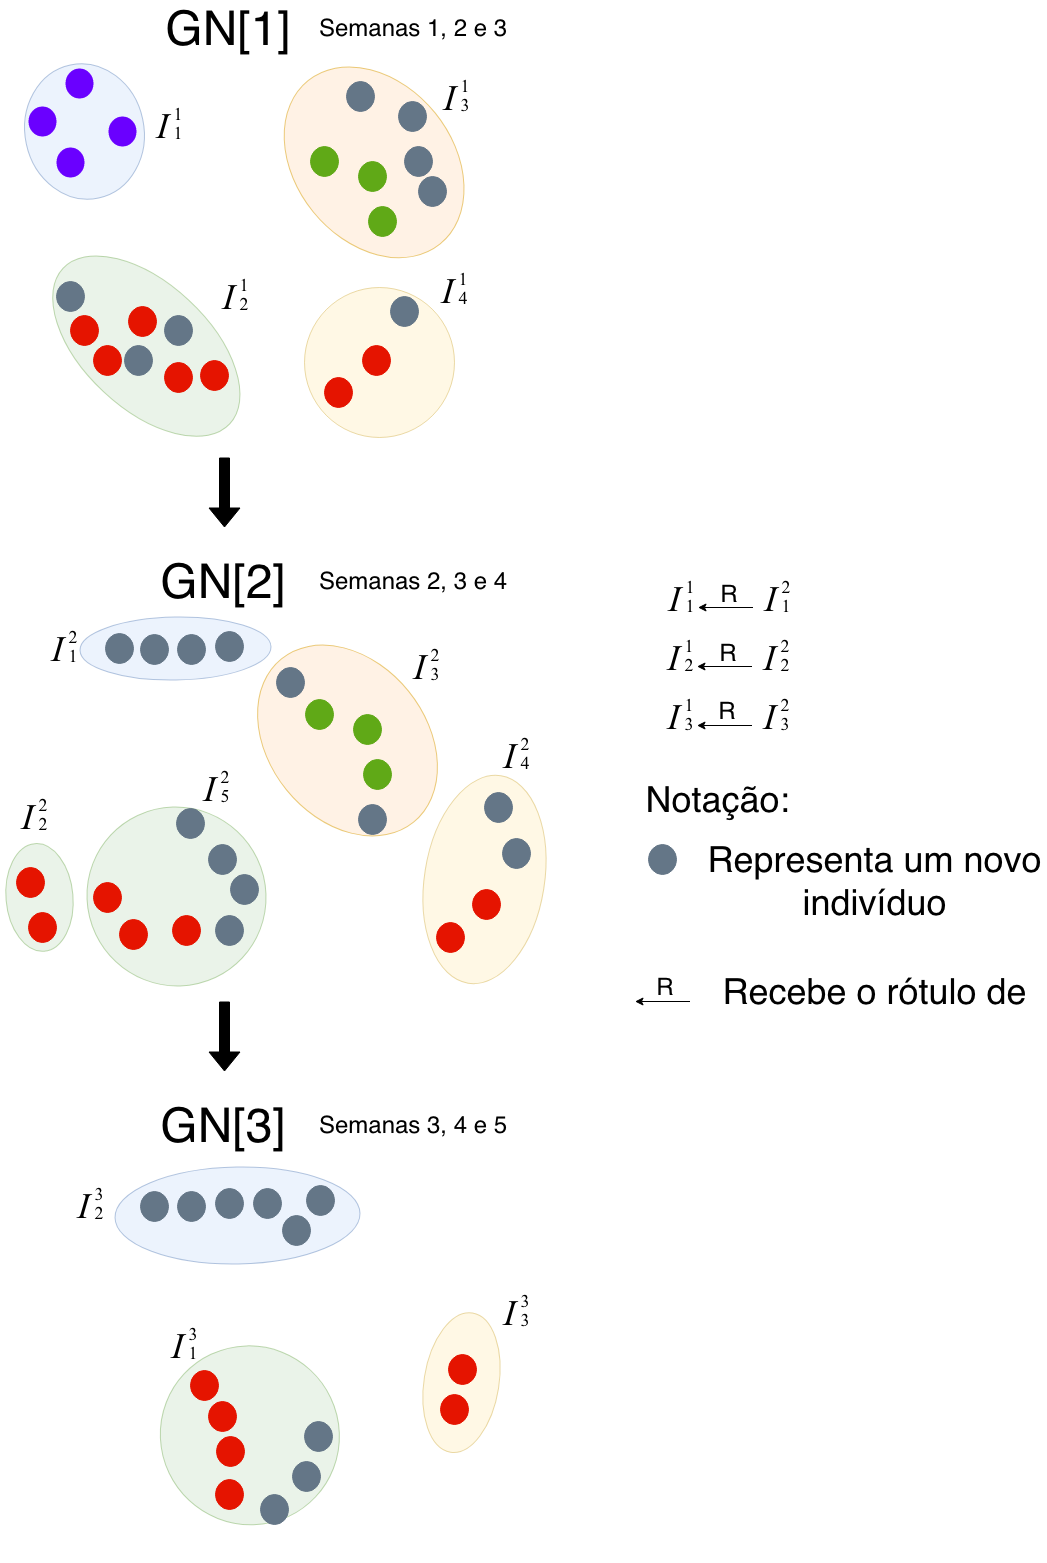
\includegraphics[width=14cm]{figuras/GN.png}
	}{
		\Fonte{Elaborado pelo autor}
	}
\end{figure}

Este procedimento foi elaborado por \cite{webdengue2008}, cujo principal objetivo era de mapear a evolução da dengue na cidade de Fortaleza, tomando como base as características de evolução dos casos e focos da doença observados em 2005 para a Regional II de Fortaleza-CE. A pesquisa se preocupou em definir intervalos de observação que justificassem um comportamento de evolução do mosquito Aedes aegypt (Focos) e dos casos humanos da doença, utilizando como ferramenta principal o algoritmo estático IGN e o \textit{framework} WebDengue \cite{webdengue2008}. Este framework é uma solução de vigilância epidemiológica composta por um conjunto de sistemas computacionais. Essas tecnologias combinam geoprocessamento, sistemas de apoio a decisão, sistemas de bancos de dados e a aquisição de dados remotos, como mostrado na figura \ref{fig:webdengue} \cite{webdengue2008}.

\begin{figure}[!ht]
	\centering
	\Caption{\label{fig:webdengue} Estrutura computacional proposta para a gestão da dengue}	
	\UECEfig{}{
		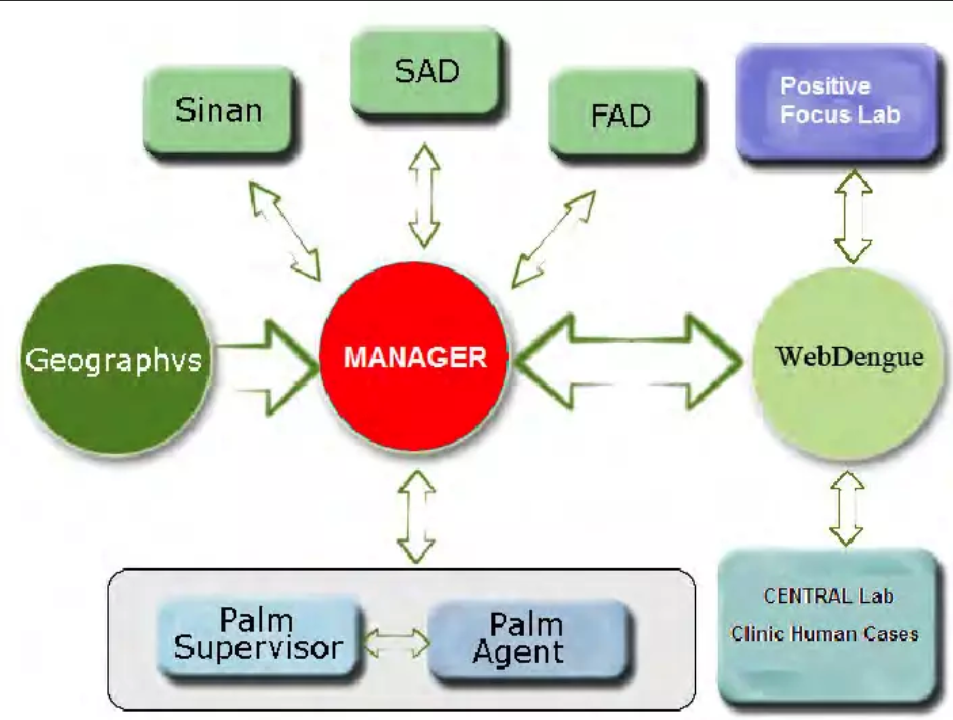
\includegraphics[width=12cm]{figuras/webdengue.png}
	}{
		\Fonte{Sistema WebDengue \cite{webdengue2011} }
	}
\end{figure}

Os dados foram tomados a partir dos informes diários de casos e focos, onde um estado é definido como o período de uma semana. Do conjunto de observações se consideram seis ternos de semana (1-2-3, 2-3-4, 3-4-5, 4-5-6) de Abril/2005 a Maio/2005 para o comportamento dos focos. Os casos são tomados para o final de cada período em razão de serem eles consequentes de possível infestação pela picada do mosquito Aedes aegypti, tomou-se então quatro quinzenas (3-4, 4-5, 5-6, 6-7) de Maio/2005 a Junho/2005 para avaliar este comportamento.

\pagebreak

\subsection{Detecção de \textit{outliers} espaço-temporais}
\textit{Outliers} são tradicionalmente definidos como instâncias que são notavelmente diferentes da maioria das instâncias no conjunto de dados. Em aplicações espaço-temporais, detectar \textit{outliers} ajuda a identificar fenômenos interessantes, mas raros, por exemplo, uma trajetória irregular tomada por um veículo de táxi ou a mudança das frequências de inundações e secas em determinadas áreas devido a mudanças climáticas ou ações humanas que mudam a ecologia de uma região \cite{Atluri:2018}.

Um aspecto a considerar por trás da detecção de \textit{outliers} espaço-temporais é que isso reflete na descontinuidade em de atributos não espaço-temporais dentro de uma vizinhança espaço-temporal \cite{cheng:2014}.

Alguns estudos descobrem \textit{outliers} considerando somente seus vizinhos temporais, enquanto outros trabalhos dizem respeito a \textit{outliers} apenas em relação a seus vizinhos espaciais. Combinando essas duas noções, um \textit{outlier} espaço-temporal (ST-Outlier) é um objeto espaço-temporal cujos atributos não-espaciais e não-temporais são significativamente diferentes dos atributos dos outros objetos em suas vizinhanças espaciais e temporais \cite{gupta:2014}.

\cite{Birant2006SpatiotemporalOD} propuseram um mecanismo de detecção ST-Outlier baseado em densidade com 3 passos:
\begin{enumerate}
    \item Agrupar usando um DBSCAN modificado. Para suportar o aspecto temporal, uma árvore é percorrida para encontrar
os vizinhos temporais de qualquer objeto dentro de um determinado raio. Para encontrar valores discrepantes quando os grupos têm diferentes densidades, o algoritmo atribui um fator de densidade a cada grupo e compara o valor médio de um grupo com o novo valor de entrada;
    \item Verificar os vizinhos espaciais para saber se esses possíveis \textit{outliers} também são \textit{outliers} espaciais;
    \item Verificar os vizinhos temporais dos \textit{outliers} espaciais.
\end{enumerate}
